\chapter{FERTILIZATION CHANGES SEAGRASS COMMUNITY STRUCTURE BUT NOT BLUE CARBON STORAGE: RESULTS FROM A 30-YEAR FIELD EXPERIMENT}		\label{another chapter}

\section{Abstract}


Seagrass ecosystems are attracting attention as potentially important tools for carbon (C) sequestration, comparable to those terrestrial and aquatic ecosystems already incorporated into climate change mitigation frameworks. Despite the relatively low C stocks in living biomass, the soil organic carbon pools beneath seagrass meadows can be substantial. We tested the relationship between soil C storage and seagrass community biomass, productivity, and species composition by revisiting meadows experimentally altered by 30 years of consistent nutrient fertilization provided by roosting birds. While the benthos beneath experimental perches has maintained dense, \textit{Halodule wrightii}-dominated communities compared to the sparse \textit{Thalassia testudinum}-dominated communities at control sites, there were no significant differences in soil organic carbon stocks in the top 15 cm. Although there were differences in $\delta$\textsuperscript{13}C of the dominant seagrass species at control and treatment sites, there was no difference in soil $\delta$\textsuperscript{13}C between treatments. Averages for soil organic carbon content (2.57 $\pm$ 0.08 \%) and $\delta$\textsuperscript{13}C (-12.0 $\pm$ 0.3 \textperthousand) were comparable to global averages for seagrass ecosystems, however our findings question the relevance of local-scale seagrass species composition or density to soil organic carbon pools in some environmental contexts.


\section{Introduction}

Organic carbon (C\textsubscript{org}) storage and flux in coastal ecosystems has been of academic interest for over two decades \citep{Smith:1981dk} but has recently undergone a revival in light of climate change mitigation efforts. Seagrass ecosystems have been identified as globally significant C\textsubscript{org} sinks \citep{Duarte:2005va, Mcleod:2011gs} with stocks comparable to terrestrial ecosystems already acknowledged for their carbon storage abilities \citep{Fourqurean:2012cv}. Understanding the environmental and ecological controls of C\textsubscript{org} stocks, particularly during environmental change, is crucial for both global carbon budgeting, and more pragmatically, mitigating greenhouse gas emissions \citep{Macreadie:2014fz}. It is clear that seagrasses can and do modify their environment in ways that promote C\textsubscript{org} storage \citep{Mateo:2006wk, Duarte:2011da}, however very seldom have these mechanisms been empirically shown to function at magnitudes and timescales that are applicable to localized disturbance regimes, climate change and global carbon cycles.

The majority of C\textsubscript{org} bound in seagrass ecosystems is stored in the soils below the seagrass meadows rather than the biomass itself \citep{Fourqurean:2012cv}. Optimal conditions for C\textsubscript{org} storage include high inputs of C\textsubscript{org} along with low or infrequent disturbance, a depositional environment and anoxic soils \citep{Duarte:2011da, Fourqurean:2012cv}. High C\textsubscript{org} input from seagrass is fueled by high productivity of seagrass meadows and typically low grazing pressure (\citealt{Westlake:1963ts, Zieman:1980wp, Enriquez:1993ul, Duarte:1996wm}; but see \citealt{HeckJr:2006km}). This direct contribution of seagrass C\textsubscript{org} to soil stock is evident from enriched soil \textsuperscript{13}C values which reflect those of seagrasses, though large portions of stored C\textsubscript{org} can be sourced to other, cohabiting marine primary producers (e.g. macroalgae and seagrass epiphytes) as well as imported (allochthonous) organic matter from other terrestrial and aquatic systems \citep{Kennedy:2010if}.

The seagrass canopy, comprised of a complex matrix of seagrass leaves, often decreases current velocity and alters the turbulence in a way that increases deposition and adds allochthonous C\textsubscript{org} to soil stocks \citep{Ward:1984vm, Fonseca:1986tz, Hendriks:2008ew}. The relative contribution of non-seagrass sources of C\textsubscript{org} to soil stocks varies greatly and can be estimated by the C isotopic composition of the soil relative to its sources \citep{Kennedy:2010if}. Generally, high ratios of \textsuperscript{13}C/\textsuperscript{12}C suggest greater seagrass input while lower ratios are indicative of non-seagrass sources like autochthonous algae or allochthonous C\textsubscript{org} from non-seagrass sources \citep{Gacia:2002tt}. Once buried, the stable, anoxic conditions of seagrass soils are thought to lead to enhanced C\textsubscript{org} preservation \citep{Duarte:2011da}. In some cases, buried organic matter can persist for millennia \citep{Mateo:1997uw, LopezSaez:2009ed}, as is the case for parts of Florida Bay (Fourqurean et al. 2012b).

These characteristics may facilitate carbon storage in seagrass ecosystems compared to unvegetated sites but it is difficult to assess their effect on long-term C\textsubscript{org} storage. In some systems, higher C\textsubscript{org} content has been found in soils underlying seagrasses compared to nearby unvegetated sediment \citep{Greiner:2013wi, Marba:2015hj, Ricart:2015cd}, while in other locations there is no clear relationship between seagrass biomass and soil C\textsubscript{org} stocks \citep{Campbell:2014cv}. Further, seagrass meadows of different species composition have been shown to vary 18-fold in C\textsubscript{org} stocks, ostensibly because of interspecific differences in rates of production, effects on sediment stabilization and environmental context \citep{Lavery:2013kh}. A common hurdle for understanding the effect of seagrasses on net C\textsubscript{org} storage is separating the effect of the seagrass community from those direct effects of the environment. In Florida Bay, \citet{Armitage:2016ek} noted a 300\% difference in regional soil C\textsubscript{org} storage across a naturally occurring productivity gradient (driven by nutrient availability) but saw no difference in soil C\textsubscript{org} content when local productivity was increased by nutrient fertilization. Differences in geomorphological and hydrological factors that control sedimentation and erosion can differ across the seascape and between patches of seagrass. Thus, simple correlations among seagrass species composition, biomass and soil C\textsubscript{org} would be confounded by such spatial variability in the sedimentary environment linked to local hydrodynamics. These environmental effects can be both confounding as well as act synergistically with seagrass communities \citep{Folmer:2012eu}.

Seagrass communities themselves could control the long-term storage of sediment C\textsubscript{org}, and thus be important to greenhouse gas mitigation efforts and global carbon budgets, if 1) seagrasses enhance the input of C\textsubscript{org} into the long-term soil carbon pool or 2) seagrasses prevent the erosion, decomposition and remineralization of the sediment C\textsubscript{org} pool that would otherwise occur. Both propositions would support the importance or seagrasses in augmenting long-term C\textsubscript{org} storage, though the latter would additionally support the importance of seagrasses to secure the globally significant soil C\textsubscript{org} stocks already in existence. Published C\textsubscript{org} burial estimates for seagrass meadows are strikingly high, however they are largely based on net primary production (NPP), short term sediment accretion studies, or a few species noted for their peat-like sediment mattes \citep{Duarte:2005va, Duarte:2010dx}. These indicators of long-term C\textsubscript{org} storage may not be generalizable to all seagrass species and locations, particularly for a large, diverse, polyphyletic group like the seagrasses.

Decomposition, in contrast to burial, is thought to occur at low rates in seagrass meadows because of stable, anoxic soils that prevent aerobic metabolism \citep{Duarte:2010dx, Fourqurean:2012cv}. Decomposing microbes may also be limited by high C:N and C:P ratios of sediment organic matter and perhaps by nutrient competition with seagrasses \citep{Enriquez:1993ul, Lopez:1995uo, Lopez:1998ty}. While issues of decomposition have been addressed in seagrass ecosystems \citep{Harrison:1989tp, Mateo:2006wk}, most studies have focused on early decomposition, rather than the altered decomposition of aged, buried C\textsubscript{org} that would be of interest to long-term carbon storage.

The aim of this study was to investigate controls of sediment C\textsubscript{org} storage over a three decade period, specifically addressing 1) whether seagrass species composition and biomass, and 2) nutrient enrichment influence sediment C\textsubscript{org} storage. To control for confounding differences in geomorphological and local hydrological factors that could directly influence C\textsubscript{org} storage, we took advantage of an experiment that has been running continuously for 31 years. The original experiment altered nutrient input, seagrass and animal community composition, rates of net primary production, and biomass within experimental blocks. We hypothesized that higher seagrass biomass would result in greater trapping and preservation of C\textsubscript{org} in sediment, but also that fertilization of seagrass meadows could relieve nutrient limitation of decomposers, resulting in decreased sediment C\textsubscript{org}. We also predicted that organic matter with higher C:N and C:P ratios would be less likely to decompose, and thus more likely to persist in sediments. This hypothesis could be supported if soil \textsuperscript{13}C signatures are more similar to those of local seagrass, particularly the carbon-rich \textit{T. testudinum}, compared with those of \textit{H. wrightii} and algae. This study addresses the controls of long-term C\textsubscript{org} storage in seagrass ecosystems, an understanding of which is vital for determining the causal relationship between seagrass ecosystems and their associated organic carbon stocks.



\section{Materials and Methods}

This study was conducted on Cross Bank (Figure~\ref{fig:map}), a shallow (<50 cm deep) carbonate mud bank in east-central Florida Bay spanning east-west from 25°00.25’ N 80°33.5’ W to 25°00.6’ N 80°36.6’ W. Cross Bank, like most of the inner regions of Florida Bay, is severely phosphorus limited  because of high N:P in freshwater runoff and low mobility of P across the landscape owing to the adsorption of P onto carbonate sediments \citep{Powell:1989tt, Powell:1991va, Fourqurean:1992we, Fourqurean:1995uj, Herbert:2008di}.  At this site, the benthos is dominated by the seagrass species \textit{T. testudinum} interspersed with \textit{H. wrightii} along with macroalgae \textit{Penicillus capitatus}, \textit{Halimeda monile}, and \textit{Laurencia} sp., with sparse presence of \textit{Batophora} sp., and \textit{Dictyota} sp. In 1981, Cross Bank was the site of a study investigating the feeding behavior of wading birds nesting on the nearby mangrove islands \citep{Powell:1985uy}. Markers were installed at 100 m intervals along the bank to serve as location references for behavioral studies, and these markers became bird perches frequented by piscivorous seabirds. Halos of dense seagrass approximately 1 - 2 m in diameter formed around the bird perches, hypothesized to be a result of nutrient input from the feces of the roosting seabirds. In 1983, this hypothesis was tested when five of the perch locations (600 m, 1200 m, 1800 m, 2400 m and 3100 m from the eastern end of Cross Bank) were selected as experimental sites \citep{Powell:1989tt}. At each of these sites, the original perch was removed. Then, two additional stakes were installed five meters from the discontinued bird perch; a new perch consisting of a wooden bock (5 cm x 10 cm x 10 cm) on top of PVC pipe (1.2 cm dia.) along with a control stake consisting of PVC sharpened to a point to prevent roosting. The resulting experimental design consisted of five sites, each with a fertilization treatment and control that has persisted for 31 years. Further site descriptions can be found in \citet{Powell:1989tt}, \citet{Fourqurean:1995uj} and \citet{Ferguson:2008fd}.

\bigskip
\noindent Sample Collection
\medskip

In February and March 2014, we collected three replicate sediment samples from experimental bird perches and their associated controls from each of the five sites. Samples were taken haphazardly from the area extending 20 cm from the PVC bird perches and control stakes. Surface soils were collected using 60 mL plastic syringes that had been modified into small piston cores (1 cm diameter, 3.0 cm depth). Deeper soil fractions were collected using a Russian Peat Borer (Aquatic Research Instruments Inc.) that produced soil cores 50 cm long by 5 cm in diameter. The extracted cores were subsampled at 10 cm (10 - 13 cm beneath surface) and 15 cm (15 - 18 cm beneath surface) by removing 3 cm core segments. The combination of methods resulted in samples from three depth fractions: 0 - 3 cm, 10 - 13 cm and 15 - 18 cm. Due to the nature of the sampling methods, soil compaction was minimized. Soils samples of known volumes were picked free of living plant tissue and stored in 18 oz pre-weighed bags (Whirlpak, Nasco), and transported to the lab for further preparation and analysis.

Surveys of seagrass standing crop (aboveground biomass) were completed in November 2014 to remain consistent and comparable with historical data. As sampling has been consistently conducted in November throughout the experiment’s 31 years, seasonal variation in seagrass biomass and well as any related ecological function is lost. Small quadrats (n = 3, 10 cm × 10 cm) were randomly placed within 30 cm of experimentally installed PVC stakes, from which all living, aboveground seagrass biomass was harvested. Seagrass leaves were separated by species, scraped of all epiphytes using a razor blade, rinsed and dried at 65 °C until a constant weight. We saw no sign of herbivory (bite or grazing marks) in the collected samples. Dried seagrass material was weighed, reported for individual species and total seagrass biomass, and compared to historic data \citep{Powell:1989tt, Powell:1991va, Fourqurean:1995uj, Herbert:2008di}. Seagrass and soil samples were collected in different seasons though our interests in long-term C\textsubscript{org} storage imply that temporary, seasonal differences in soil composition can be disregarded. Dry samples of each species were pooled within each replicate, homogenized and ground to a fine powder using a motorized mortar and pestle in preparation for stable isotope analysis.

\newpage


\noindent Soil Analyses
\medskip


Soil samples were analyzed for dry bulk density, organic and elemental content (C, N, P) as well as C\textsubscript{org} content and $\delta$\textsuperscript{13}C. Soil samples of known volumes were stored on ice in pre-weighed sample collection bags until they were dried at 65 °C for a minimum of 48 hours to obtain a dry weight. Dry bulk density (DBD) was calculated as the dry weight of the soil divided by the volume of the original soil sample and expressed as gram dry weight per cubic centimeter.

The dried soil samples were homogenized and ground to a fine powder using a motorized mortar and pestle. Powdered samples were analyzed for total carbon (TC) and nitrogen content using a CHN analyzer (Fisons NA1500). Given the high calcium carbonate content of Florida Bay soils \citep{Bosence:1989wi}, it was necessary to account for the inorganic carbon (C\textsubscript{inorg}) in the soil samples in order to measure C\textsubscript{org}. Subsamples of dried material were weighed, ashed at 500 $^{\circ}$C for five hours and reweighed, enabling organic content to be calculated as loss on ignition (LOI). To measure the C\textsubscript{org} content of the soil samples, we used the instrumental analyzer-dry oxidation procedures described by \citet{Fourqurean:2012hu}. In brief, ashed soil samples remaining after the LOI technique were reanalyzed using a CHN analyzer to quantify the C\textsubscript{inorg}. The C\textsubscript{inorg} content of the ash was used to calculate the C\textsubscript{org} as TC - C\textsubscript{inorg} after scaling C\textsubscript{inorg} back to the original soil weight using LOI. Though there is a correlation between LOI values and \% C\textsubscript{org} \citep{Fourqurean:2012cv}, only values of C\textsubscript{org} are presented here. Phosphorus content was determined by a dry-oxidation, acid hydrolysis extraction followed by a colorimetric analysis of phosphate concentration of the extract \citep{Fourqurean:1992we}. Elemental content of phosphorus in soil samples was calculated on a dry weight basis.

\newpage

\noindent Stable Isotope Analysis
\medskip


	Dry, homogenized samples of seagrasses and soil (0 and 15 cm depth fractions only) from each replicate were fumed with HCl for >7 days prior to isotopic analyses to remove associated carbonates. Samples were then redried and analyzed for $\delta$\textsuperscript{13}C using standard elemental analyzer isotope ratio mass spectrometer (EA-IRMS) procedures. The elemental analyzer was used to combust the organic matter and to subsequently reduce the formed carbon-containing gases to CO\textsubscript{2}, which was then measured on a Finnigan MAT Delta C IRMS in a continuous flow mode. These results are presented with respect to the international standards of Vienna Pee Dee belemnite (V-PDB) for carbon using the secondary standards IAEA CH-6 for $\delta$\textsuperscript{13}C. Analytical reproducibility of the reported $\delta$ values was better than $\pm$ 0.08 for $\delta$\textsuperscript{13}C, based on sample replicates.

\bigskip
\noindent Data Analysis
\medskip

	The average aboveground biomass values of the three quadrats at each experimental replicate were used in statistical analyses. The effect of bird perch on total aboveground biomass as well as seagrass species specific weight contributions were assessed using a repeated measures analysis of variance with treatment (bird perch vs control) as the within-subject factor. Each site (consisting of one experimental set of stakes) constituted a subject in these analyses. The procedure was run separately for total biomass and species-specific contributions to total biomass $\delta$\textsuperscript{13}C values of \textit{T. testudinum} and \textit{H. wrightii} leaf tissue were analyzed for treatment effects using a similar ANOVA. Data containing unequal variances were tested using Friedman’s or Mann–Whitney–Wilcoxon tests depending if subjects were included.

	Sediment cores from each PVC stake (n = 3) were averaged for each replicate prior to statistical investigation. Differences in soil characteristics as a function of both treatment and depth were assessed using mixed-model univariate repeated measures analysis of variance with treatment and depth fraction as within-subject factors. Each site (consisting of one experimental set of stakes) constituted a subject in these analyses. Four of these ANOVAs were run; one for each nitrogen, phosphorus, $\delta$\textsuperscript{13}C and C\textsubscript{org} content of the soil. If data for any analysis did not meet one of the test’s distribution-based assumptions, a Friedman's test for a randomized complete block design was used, classifying each subject as an experimental block. Treatment effect was then tested for each depth fraction.

	Soil C\textsubscript{org} content data was then compared to seagrass standing crop for each replicate for the two dominant seagrasses, \textit{H. wrightii} and \textit{T. testudinum}, as well as total seagrass standing crop using a Model II Linear Regression due to the error associated with both variables. This test was performed three times, once for each seagrass species as well as total aboveground biomass. A similar Model II Regression was used to test for a relationship between soil carbon density (mg C\textsubscript{org} cm\textsuperscript{-3}) and the measured benthic community variables. Differences in soil $\delta$\textsuperscript{13}C between depth fractions and treatments were tested using ANOVA or Mann–Whitney–Wilcoxon procedures after data were checked for normality and equal variances.


\section{Results}

	Differences in aboveground seagrass biomass at treatment and control plots were similar to those previously reported \citep{Powell:1991va, Fourqurean:1995uj, Herbert:2008di} with aboveground biomass from \textit{H. wrightii} significantly higher at bird perch treatments compared to control sites (Figure~\ref{fig:1fig1}; ANOVA, p < 0.05) with a mean difference of 92.0 $\pm$ 15.5 g m\textsuperscript{-2}. Bird perches and controls did not show a significant difference in \textit{T. testudinum} aboveground biomass (p > 0.05), likely due to a single leverage point (Figure~\ref{fig:1fig1}). However there were significantly lower contributions of \textit{T. testudinum} to total aboveground biomass from the bird perch treatments compared to control treatments with a mean difference of 79.0 $\pm$ 12.6 \%. Despite the documented effect of bird perches on aboveground biomass for individual species, differences between total aboveground seagrass biomass have not been consistent over the history of the experimental plots. Our sampling did not show a statistical difference between total aboveground biomass at the bird perch treatment and control sites when we sampled (ANOVA, p > 0.05).

\bigskip
\noindent Soil Characteristics
\medskip


	Dry bulk density (DBD) on Cross Bank was 0.59 $\pm$ 0.02 g mL\textsuperscript{-1} and remained indistinguishable between bird perch and control sites with a mean difference of 0.00 $\pm$ 0.04 g mL\textsuperscript{-1} (ANOVA, p>0.95). There were, however, differences in DBD between five experimental blocks (ANCOVA, p < 0.05) with an average DBD ranging between 0.48 and 0.69 g mL\textsuperscript{-1} for sites with the most extreme soil densities (Figure~\ref{fig:1fig2}). DBD on average was lowest in surface soils, increasing down core by 0.01 g mL\textsuperscript{-1} per cm of core depth. DBD was negatively correlated with C\textsubscript{org} and N across the sites (Figure~\ref{fig:1fig3}, linear regression, p < 0.05). There was a positive correlation between soil C\textsubscript{org} and N content (Figure~\ref{fig:1fig4}) though no correlation between soil P content and C\textsubscript{org} content. DBD in surface soils showed a positive correlation with proximity to inhabited land (linear regression, p < 0.05).

	The fertilization effect from roosting birds can be seen throughout the first 15 cm of soil with an average soil phosphorus content of 992 $\pm$ 341 μg P g\textsuperscript{-1} at experimental bird perch plots compared to control plots of 64 $\pm$ 25 μg P g\textsuperscript{-1} and the Florida Bay average of 99.5 $\pm$ 20.0 μg g\textsuperscript{-1} \citep{Fourqurean:2012hu}. Sediment phosphorus was significantly different between bird perches and controls for all depth fractions (Friedman’s test, p < 0.05). Within the bird perch treatments, there was no significant correlation between soil depth and phosphorus concentration (ANOVA, p > 0.05), and soil phosphorus concentrations for bird perch treatments exhibited different down-core patterns between sites (Figure~\ref{fig:1fig5}) ranging from consistently low P concentrations at Site 1, to differences in down-core soil P concentrations that range over two orders of magnitude (Sites 4 and Site 5).

	Soil nitrogen content was slightly higher at bird perch treatments than controls (0.27 $\pm$ 0.01 \% of dry weight and 0.25 $\pm$ 0.01 \%, respectively; Figure~\ref{fig:1fig6}; ANOVA, p < 0.05), but this slight difference was negligible. We also noted a varying N content of soils between the five sites; N content increased with proximity to inhabited land (linear regression, p < 0.05), ranging from an average of 0.29 \% N at site 1 to an average of 0.23 \% at site 5 but was also decreased with soil DBD (linear regression, p < 0.05). There was no effect of soil depth on N content (ANOVA, p > 0.05).

	C\textsubscript{org} content of the soil samples averaged 2.57 $\pm$ 0.08 \% of dry weight across all samples collected, ranging between 1.12 to 4.64 \% of dry weight. These values fall near the global mean of 2.5 $\pm$ 0.1 \% and the more commonly used median of 1.8 \% \citep{Fourqurean:2012cv}, as well as the average value reported for Florida Bay of 2.1 $\pm$ 0.3 \% \citep{Fourqurean:2012hu}.

	Long-term fertilization changed the nature of the seagrass community in our study site from \textit{T. testudinum}- dominated to \textit{H. wrighii}-dominated however, there were no significant differences in soil C\textsubscript{org} content between these two benthic community types (Figure~\ref{fig:1fig7}; ANOVA, p > 0.05). Similarly, there were no significant differences in C\textsubscript{org} density (measured as g C\textsubscript{org} mL\textsuperscript{-1}) between controls and experimental plots. There were, however, significant differences in C\textsubscript{org} content between the study sites (Figure~\ref{fig:1fig8}, ANOVA between subject, p < 0.05). Site 1 had the highest average C\textsubscript{org} content (2.95 $\pm$ 0.06 \% of dry weight), while Site 5 had on average the lowest C\textsubscript{org} content (2.12 $\pm$ 0.17 \% of dry weight) throughout the core. A significant depth effect was not observed (ANOVA, p > 0.05). These trends correlate with soil DBD across the five sites.

	Densities of both \textit{H. wrightii} and \textit{T. testudinum} varied within both perch and control sites. Ignoring the experimental setup, linear models were constructed between seagrass densities and their respective surface soil C\textsubscript{org} content including data from both experimental and control plots (Figure~\ref{fig:1fig9}). There was no evidence for a correlation between \textit{H. wrightii}, \textit{T. testudinum}, or total seagrass aboveground biomass with C\textsubscript{org} content in surface soils (Model II Linear Regression, P > 0.1). Similarly, there was no correlation between soil C\textsubscript{org} stock in the first 3 cm and any of the measured benthic community variables (Model II Linear Regression, P > 0.1).

\bigskip
\noindent Carbon Stable Isotope values of seagrasses and soil C\textsubscript{org}
\medskip



	\textit{T. testudinum} leaves ($\delta$\textsuperscript{13}C  = –8.4 $\pm$ 0.3 \textperthousand) were more enriched in \textsuperscript{13}C than \textit{H. wrightii} (–9.8 $\pm$ 0.4 \textperthousand; ANOVA, p < 0.05, Figure~\ref{fig:1fig10}). Seagrass $\delta$\textsuperscript{13}C was not affected by fertilization or site for either species (ANOVA, p > 0.05). The $\delta$\textsuperscript{13}C of soil C\textsubscript{org} averaged -12.0 $\pm$ 0.3 \textperthousand, and ranged between -10.7 \textperthousand{} and -15.4 \textperthousand. There was no effect of treatment nor site on the soil $\delta$\textsuperscript{13}C (ANOVA, p > 0.05). There was however a difference in $\delta$\textsuperscript{13}C between surface soil and the 15 cm depth fraction (Figure~\ref{fig:1fig9}; Mann–Whitney–Wilcoxon, p < 0.05) with surface soil being on average 1.5 \textperthousand{} more depleted. Variance was also lower in surface soils compared to 15 cm fraction (Levene’s test, p < 0.05).


\section{Discussion}

	Over the 30 years since experimental bird perches were installed on Cross Bank, they have provided insight on the feeding behavior of seabirds \citep{Powell:1985uy}, nutrient limitation and the nature of competition in seagrasses \citep{Powell:1989tt, Powell:1991va, Fourqurean:1995uj}, the effect of eutrophication on mollusk diversity in seagrass beds \citep{Ferguson:2008fd}, and long-term ecosystem effects of short and long-term nutrient enrichment \citep{Herbert:2008di}. After the three decades, the experimental plots also provided a novel setting for investigating the relationship between seagrass communities and long-term soil storage of C\textsubscript{org}. Despite extreme, consistent differences in nutrient availability, net primary production and seagrass community structure between bird perch treatments and control (herein called \textit{Halodule}-dominated and \textit{Thalassia}-dominated, respectively) sites over three decades, there was no difference in C\textsubscript{org} storage in the top 15 cm of underlying soil. Varying morphologies, elemental stoichiometry, metabolism and wave attenuation capabilities exist between fertilized and control plots and between the dominant species, yet there were no differences in the content or density of C\textsubscript{org} in the soils. There were, however, differences in the C\textsubscript{org} soil storage between experimental blocks over the 3.6 km environmental gradient that they span.

\bigskip
\noindent The Seagrass – Soil C\textsubscript{org} Link
\medskip

	The most direct way that seagrasses contribute to soil C\textsubscript{org} storage is through the burial and preservation of its biomass in the underlying soil (see \citealt{Holmer:2009tj}). Seagrass biomass itself contributes a global average of 50 \% of the total stored soil C\textsubscript{org}, though the tendency for a plant, or portion of the plant, to be stored can vary greatly due to environmental factors \citep{Kennedy:2010if}. For example, seagrass leaves can contribute more to local C\textsubscript{org} carbon stores than rhizomes \citep{Kennedy:2010if} yet are more likely to move laterally from its origin due to water currents and the buoyancy of leaves \citep{Zieman:1979ui}. A significant fraction of seagrass biomass and production is positioned in belowground structures, accelerating the process of burial of seagrass-derived C\textsubscript{org}. While this belowground plant material can be eroded out of the soil after death, its alternative fates are in situ decomposition or preservation. The quantity and molecular composition of buried organic material as well as its environmental setting all affect its preservation \citep{Harrison:1989tp, Arndt:2013bc}; all of these factors vary between \textit{Thalassia}-dominated and \textit{Halodule}-dominated sites.

	While total aboveground biomass was indistinguishable between \textit{Thalassia}-dominated plots and \textit{Halodule}-dominated plots for the majority of the years sampled, belowground morphology varies between the species. \textit{H. wrightii} belowground biomass at Cross Bank consists of only 44 - 60 \% of total plant mass compared to over 70 \% for \textit{T. testudinum} \citep{Powell:1989tt}. Further, the ratio of thick, structurally complex rhizome to root biomass is almost twice as much for \textit{T. testudinum} \citep{Duarte:1998uz}. This difference in belowground allocation among species could help explain the lack of differences in soil C\textsubscript{org} stores between dense, \textit{Halodule}-dominated and more sparse \textit{Thalassia}-dominated seagrasses on Cross Bank.

	When seagrasses are relieved from nutrient limitation, they allocate less of their production to building belowground biomass \citep{Gleeson:1993wj, Lee:2000cn}. Exemplifying this trend, \citet{Powell:1989tt} noted that those \textit{T. testudinum} plants that remain at the \textit{Halodule}-dominated plots have less belowground biomass compared to those at \textit{Thalassia}-dominated plots (74 – 88 \% and 80 – 98 \% total biomass, respectively). There is less belowground biomass at \textit{Halodule}-dominated plots, with both inter- and intra-species differences that can alter soil C\textsubscript{org} influx.

	The rate and extent of decomposition for seagrass-derived organic matter is considered to be greatest in an oxidized water column and surface sediments where aerobic respiration can yield higher bacterial production rates \citep{Harrison:1989tp, Arndt:2013bc}. In Florida Bay, sediments inhabited by seagrasses are depleted of oxygen within the upper 5 mm of the sediment with decreasing concentrations along the depth profile \citep{Borum:2005if}. Though seagrasses can release oxygen into soil from their roots through advective exchange, bulk soil oxygen concentrations beneath seagrasses is zero compared to measurable concentrations in bare sediments \citep{Burdige:2002to, Holmer:2009tj}, and any microzones of oxygen release around the roots are so small as to be indistinguishable using a 500 µm microelectrode \citep{Borum:2005if}. \textit{T. testudinum} roots and horizontal rhizomes are on average deeper (approximately 15 cm) than those of \textit{H. wrightii} which penetrate only a few centimeters \citep{Duarte:1998uz}. These trends also hold true at Cross Bank (personal observation) with horizontal rhizomes of \textit{H. wrightii} (typically considered belowground biomass) observed to extend 20 - 30 cm up into the water column \citep{Fourqurean:1995uj}.

	The nutrient content of plant-derived organic matter can influence the rate of decomposition, with higher N and P content resulting in more rapid decomposition rates \citep{Enriquez:1993ul}. The fertilization experiments utilized in this study altered the elemental stoichiometry of seagrasses, lowering the C:P ratio of both leaf and rhizome biomass \citep{Herbert:2008di, Powell:1989tt}, and by adding P to a severely P-limited ecosystem \citep{Fourqurean:1992we}. There is some evidence that heterotrophic soil-inhabiting bacteria that remineralize detritus can be P-limited in carbonate sediments \citep{Lopez:1995uo, Lopez:1998ty}, thus relieving bacteria from limitation via enriched detritus and loaded phosphate could increase bacteria production and decomposition rates; yet we found no differences in soil C\textsubscript{org} between fertilized and non-fertilized, P-poor plots.

	All of the aforementioned trends would suggest greater decomposition and remineralization rates in \textit{Halodule}-dominated sites. \citet{Herbert:2008di} noted ecosystem respiration rates 1.6 times higher for the \textit{Halodule}-dominated plots, though measured net ecosystem production was shown to be five times greater on average at \textit{Halodule}-dominated sites compared to the \textit{Thalassia}-dominated sites. Net autotrophy could lead to the accumulation of organic matter, but differences in accumulated soil C\textsubscript{org} are limited to between depth fractions and sites rather than between seagrass community types on Cross Bank. There was no consistent difference in total aboveground biomass between benthic community types at our sites, and based on species-specific morphology, there is likely more belowground biomass at \textit{Thalassia}-dominated plots. Seagrasses are known to exude large portions of their primary production as DOC \citep{Ziegler:1999wx}. This may account for some of the differences in net production however this exudate is likely too labile to be relevant in soil C\textsubscript{org} storage. There are other factors on Cross Bank, primarily export, that could account for the discrepancy between community-specific net ecosystem production and accumulated C\textsubscript{org}.

	Globally, approximately 50 \% of the C\textsubscript{org} contained in seagrass soil pools is not of seagrass origin \citep{Gacia:2002tt, Kennedy:2010if}. Rather, it is a combination of imported, non-seagrass material (both terrestrial and aquatic) and autochthonous algal C\textsubscript{org}  that accumulates in seagrass meadows due to the altered hydrodynamic environment and additional substrate provided by seagrasses. \textit{Zostera marina} (structurally comparable to \textit{T. testudium}) seagrass canopies have been shown to reduce near-bottom mean velocities by 70 to 90 \%, while wave heights were reduced 45 to 70 \% compared to adjacent unvegetated regions \citep{Hansen:2012gl}. The fraction of the suspended particles deposited in the benthos is dependent on the settling speed of the suspended particles in relation to the upward force caused by water currents. It is the absolute water velocity (often decreased by the seagrass canopy) combined with the particle size and type that controls sedimentation \citep{Boer:2007ch}.

Altered flow is generally thought to cause net deposition of C\textsubscript{org} in seagrass meadows, contributing to underlying soil C\textsubscript{org} pools \citep{Kennedy:2010if, Fourqurean:2012cv}, however this phenomena only occurs when the attenuation effects of seagrass decrease local water velocity below the threshold for deposition. While the canopies of \textit{Thalassia}- vs \textit{Halodule}- dominated plots have different soil capturing abilities due to differing aboveground structure \citep{Mellors:2002vi, Boer:2007ch}, these factors may have little influence if the local regional water velocity is too fast to allow for sedimentation, even when the current attenuation effects of seagrass canopies are considered. For example, \citet{Hansen:2013fn} found that the current threshold required to induce soil suspension in Zostera meadows was surpassed 80 – 85 \% of their sampling period in the winter and 55 \% of the time in the summer. This can be compared to an unvegetated site, where this threshold was surpassed 90 \% of the time across all seasons. While there is often more sedimentation and less soil suspension in seagrass meadows, local water velocity ultimately controls these factors. Our biomass measurements for Cross Bank are limited the autumn, so comments regarding site-specific seasonally would be unsupported. However, fall and winter have the lowest leaf emergence rates, standing stocks and productivity in Florida Bay \citep{Zieman:1999uj, Peterson:2001wu}. The potential hydrodynamic effects of seasgrasses are likely to be more pronounced during other seasons. Neither water velocity, wave frequency, nor shear stress were measured during this study, though we could use dry bulk dry density as an indicator of hydrologic stress on the sea bottom with lighter, less dense sediments indicative of low bottom stress. There was no difference in soil dry bulk density between the \textit{Thalassia}- and \textit{Halodule}-dominated plots, possibly due to similar hydrologic regimes. This could explain the similar soil C\textsubscript{org} stocks between treatments. Rather than increased sedimentation and C\textsubscript{org} storage in \textit{Thalassia}-dominated plots, we could expect sedimentation and suspension to correlate more with local hydrological patterns than the benthic community density or assemblage. As further support, we noted differences in bulk densities between our five sites, hinting at differences in local depositional environments. As dry bulk density correlates negatively with C\textsubscript{org} in Florida Bay, there is a tendency for higher C\textsubscript{org} content at sites with lower dry bulk densities.

If the input of seagrass tissue itself is driving the C\textsubscript{org} storage in seagrass soils, it is expected that there would be a correlation between seagrass community and soil $\delta$\textsuperscript{13}C. Surface soil C\textsubscript{org} on Cross Bank was between 1.42 \textperthousand{} and 3.18 \textperthousand{} more enriched in \textsuperscript{13}C than values predicted using global models \citep{Kennedy:2010if}. This enrichment suggests that there is a greater contribution of seagrass-derived C\textsubscript{org} to the soils of Florida Bay than the global average. This high seagrass C\textsubscript{org} in the soil may be related to exceptionally high quantities of seagrass C\textsubscript{org} input on Cross Bank influencing soil C\textsubscript{org} stocks proportionally greater than other seagrass meadows. Alternatively, and more likely, it is due to the isolation of the bank from allochthonous inputs like terrestrial plants and anthropogenic sources that can be found closer to inhabited islands and mainland Florida. Cross Bank is located in an oligotrophic region of Florida Bay, 2.5 km from the nearest inhabitable island, thus algal contributions to soil C\textsubscript{org} are likely low as well. \textit{T. testudinum} and \textit{H. wrightii} have different $\delta$\textsuperscript{13}C values on Cross Bank, confirming species-specific values across Florida Bay \citep{Campbell:2009fi}. If seagrasses are important C\textsubscript{org} sources to their localized underlying soils, then we would predict that the $\delta$\textsuperscript{13}C of surface soils would reflect that of the dominant species inhabiting the area. We found that the $\delta$\textsuperscript{13}C - C\textsubscript{org} of surface soils were indistinguishable between \textit{Thalassia}- and \textit{Halodule}-dominated plots, despite the clear differences in $\delta$\textsuperscript{13}C of their dominant seagrass species. We interpret this as a homogenization of soil organic matter (dead plant material, detritus, soil) within the region of Cross Bank. Rather than C\textsubscript{org} remaining in situ, we hypothesize that repeated resuspension and transport allows mixing to occur within the spatial scale of our sites. This could also explain the similarities in soil C\textsubscript{org} content between the two seagrass community types. Morphology and sediment characteristics of banks are shaped by water movement and direction in Florida Bay and given the courser grain size found on banks compared to basins we can infer periods of greater sediment suspension \citep{Bosence:1989tx}. Once buried, C\textsubscript{org} undergoes diagenetic alteration that suggests a persistence of seagrass-derived C\textsubscript{org} relative to other sources, as indicated by the higher $\delta$\textsuperscript{13}C values of the organic matter at 15 cm compared to surficial samples.

\bigskip
\noindent Implications for Conservation and Blue Carbon Policies
\medskip

The amount of C\textsubscript{org} stored in soils under seagrass meadows is large enough to be factored into global carbon budgets \citep{Fourqurean:2012cv} and while efforts are underway to integrate seagrass soil C\textsubscript{org} into climate change mitigation efforts \citep{Duarte:2010dx, Duarte:2011da, Mcleod:2011gs}, a thorough understanding of soil C\textsubscript{org} storage is admittedly lacking \citep{Pendleton:2012hz, Macreadie:2014fz}. Seagrass coverage and production have been linked causally to the long-term soil C\textsubscript{org} stores in the literature \citep{Duarte:2010dx, Duarte:2011da}, and researchers postulate that seagrass expansion will lead to increased C\textsubscript{org} stores \citep{Duarte:2013ks} and meadow destruction will lead to increased remineralization \citep{Pendleton:2012hz, Fourqurean:2012cv}. These claims, however, have limited empirical support.

There have been case studies where seagrass recolonization and expansion have increased local soil C\textsubscript{org} stores \citep{Greiner:2013wi, Marba:2015hj} but this is not always the case \citep{Pedersen:1997fo}. \citet{Lavery:2013kh} have shown geographic variability in seagrass soil C\textsubscript{org} stores in coastal Australia but they have methodologically linked the variation to seagrass species. While morphological and physiological differences between species can account for some of the difference in C\textsubscript{org} stores, \citet{Lavery:2013kh} point out that environmental differences like hydrology and temperature have direct influences on both the species present as well as net C\textsubscript{org} storage. \citet{Serrano:2014ho} found that water column depth decreases seagrass soil C\textsubscript{org} storage likely due to the negative effects of decreased light availability on seagrasses and cohabiting primary producers. However, they also suggest that environmental factors like soil accretion and depositional environment are drivers of C\textsubscript{org} storage. \citet{Armitage:2016ek} found that soil C\textsubscript{org} content is positively related to long-term, landscape-wide trends in nutrient availability and productivity but short-term fertilization within regions of Florida Bay did not influence soil C\textsubscript{org} content, despite its effects on production and seagrass standing stock. These points of environmental context, while generally overlooked in Blue Carbon literature, may have important implications for understanding soil C\textsubscript{org} dynamics in vegetated coastal areas. Also, putting our results in the context of the work of \citet{Armitage:2016ek}, we may lack the large spatial scale changes required to alter soil C\textsubscript{org} stores. If soil C\textsubscript{org} is homogenized with the Cross Bank region of Florida Bank as suggested, then small scale increases in C\textsubscript{org} at \textit{Halodule}-dominated sites would be diluted across the larger, less-productive area and bulk changes in C\textsubscript{org} storage would be undetectable. On the other hand, regional increases in productivity could translate in to notable differences in soil C\textsubscript{org} storage. Our work also confirms that there are drivers beyond the density, productivity, and species composition of seagrass meadows controlling C\textsubscript{org} storage. Minor differences in geographic location can lead to differences in sedimentary environments across seagrass landscapes, interacting with and possibility overriding the effects of the seagrass meadow itself on C\textsubscript{org} storage.

Conservation of seagrasses is important for established reasons such as nutrient cycling and providing nursery grounds for a variety of animals \citep{Costanza:2014ex, Hejnowicz:2015fa}, but the relationship between Blue Carbon stores and seagrasses is a complicated issue that includes species-specific characteristics and environmental contexts. Beyond the academic understanding of C\textsubscript{org} storage and preservation, the current methods for assessing the Blue Carbon value of seagrass ecosystems are inadequate. On Cross Bank, the typical Blue Carbon accounting method of sediment coring would miss the differences in net ecosystem production (thus differences of CO\textsubscript{2} consumption) that have been reported between our experimental treatments. Organic carbon inputs in Florida Bay are dominated by seagrass-derived material, however the location and extent of preservation can be decoupled from its source, owing its storage and persistence to a combination of biological and environmental factors. Understanding these interactions and how to properly quantify seagrass contribution to carbon sequestration will prioritize and evaluate the worth of seagrass C\textsubscript{org} stocks, both ecologically and economically.


\section{Acknowledgements}

This chapter was published in \textit{Estuaries and Coasts} with coauthors Christian Lopes, Alex Perez, and James Fourqurean. This research was funded by the US Environmental Protection Agency as part of the Florida Keys National Marine Sanctuary Water Quality Protection Program (Contract No. X7 95469210) and by the National Science Foundation through the Florida Coastal Everglades Long-Term Ecological Research program under Grant No. DEB-1237517. Philip Matich provided invaluable lab assistance. Along with Philip, this project was enriched by Jean Alcazar and three anonymous reviewers who offered support and valuable comments. This is contribution number 759 of the Southeast Environmental Research Center at FIU.

\section{\normalfont{Work Cited}}
\begingroup

\setlength{\bibsep}{10pt}
\linespread{1}\selectfont

\renewcommand{\section}[2]{}%
\bibliographystyle{apalike}
\bibliography{wholebib1}
\endgroup


\begin{figure}
  \centering
  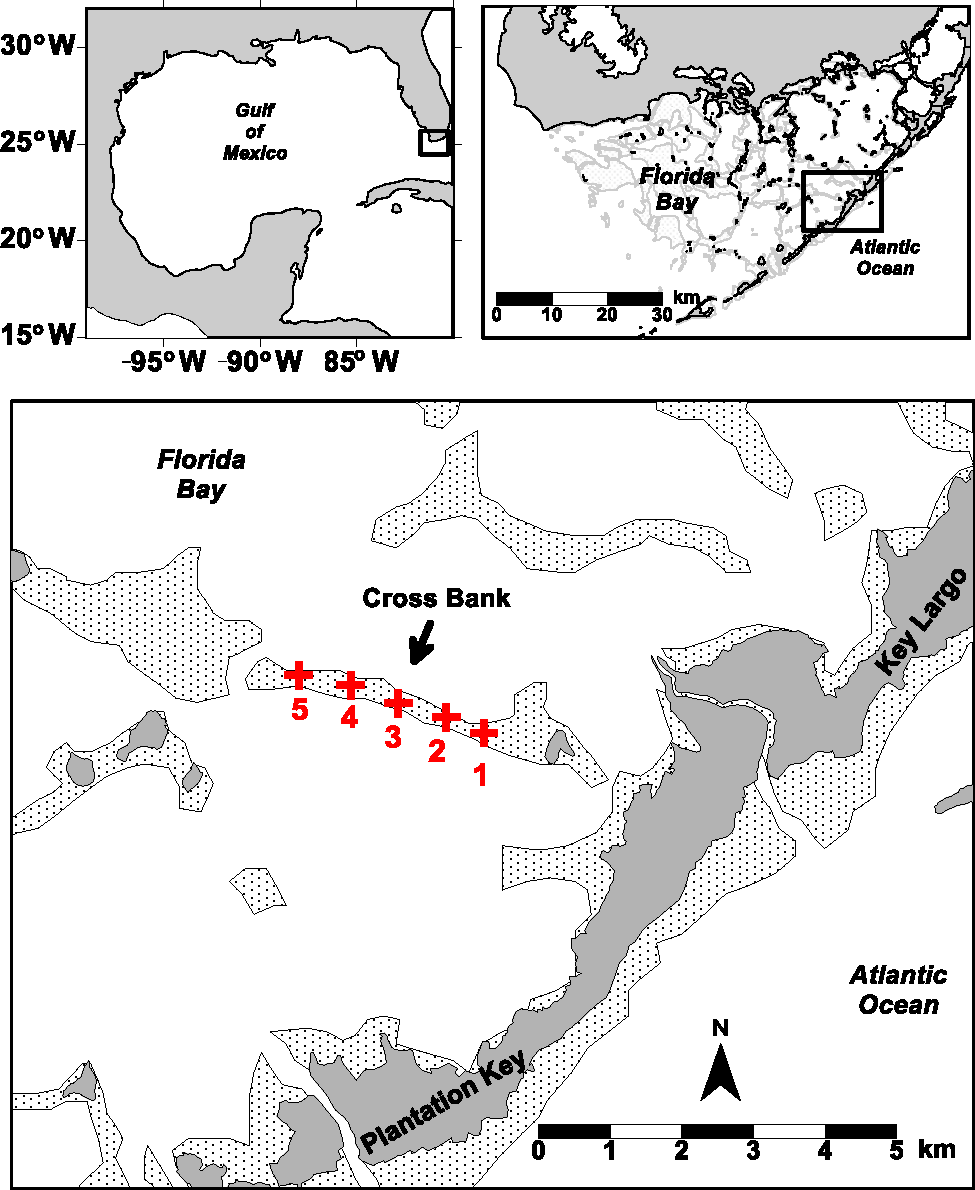
\includegraphics[width=.99\textwidth]{Figures/chapter1/chart1map}
\caption[Study area showing locations of experiment sites along Cross Bank, Florida Bay. Each site, denoted by a cross, has both an experimental bird perch and a control spaced 10 meters apart]{Study area showing locations of experiment sites along Cross Bank, Florida Bay. Each site, denoted by a cross, has both an experimental bird perch and a control spaced 10 meters apart.}
  \label{fig:map}
\end{figure}


\begin{figure}
  \centering
  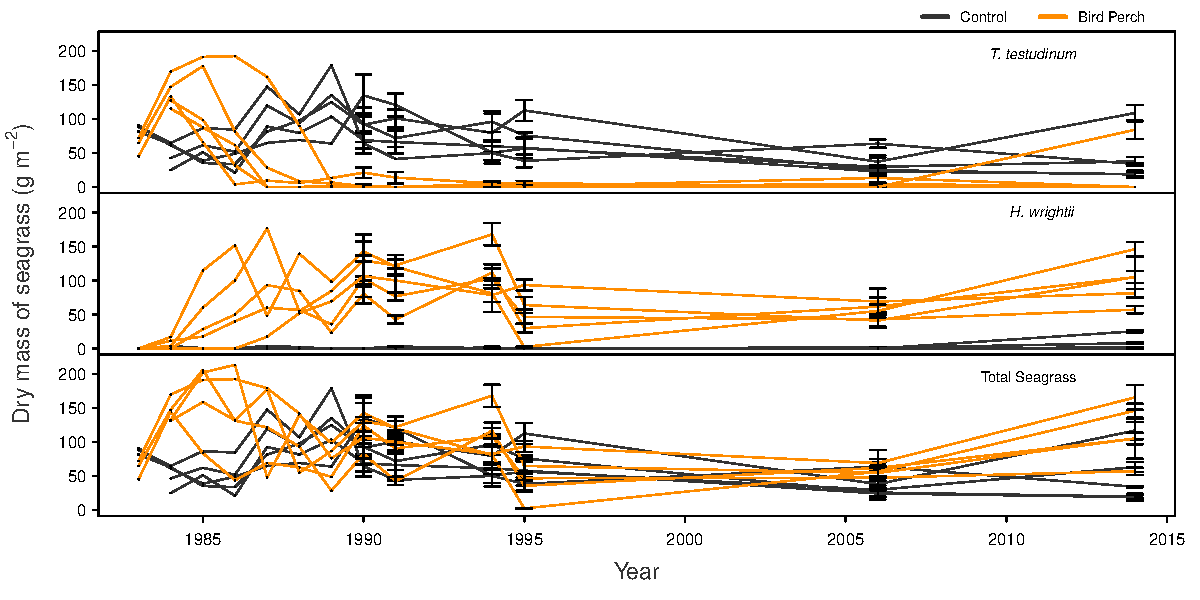
\includegraphics[width=.99\textwidth]{Figures/chapter1/fig1}
\caption[Changes in seagrass species composition showing shifts in dominance between \textit{T. testudinum} (first panel) and \textit{H. wrightii} (second panel) under conditions of long-term continuous fertilization compared to control. Total mass of seagrass however showed no clear shift under fertilization treatment (third panel). Data represents mean $\pm$ SE (N = 3, within-site replicates) of aboveground biomass with the exception of data collected prior to 1990 that lacked replicates]{Changes in seagrass species composition showing shifts in dominance between \textit{T. testudinum} (first panel) and \textit{H. wrightii} (second panel) under conditions of long-term continuous fertilization compared to control. Total mass of seagrass however showed no clear shift under fertilization treatment (third panel). Data represents mean $\pm$ SE (N = 3, within-site replicates) of aboveground biomass with the exception of data collected prior to 1990 that lacked replicates.}
  \label{fig:1fig1}
\end{figure}

\begin{figure}
  \centering
  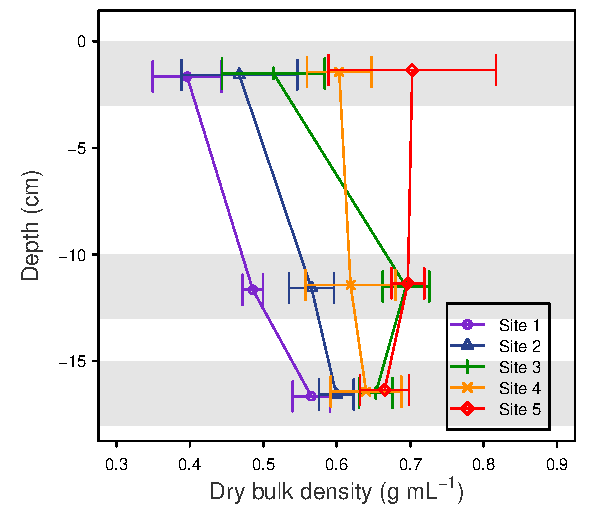
\includegraphics[width=.95\textwidth]{Figures/chapter1/fig2}
\caption[Down core profiles of dry bulk density for the five sites (treated as experimental blocks), spaced 600 m apart on Cross Bank, Florida Bay. Points represent mean of samples taken from both experimental and control treatments within each site. Horizontal error bars represent $\pm$ SE (N = 6). Grey horizontal bars represent the depth range sampled and homogenized for soil analyses]{Down core profiles of dry bulk density for the five sites (treated as experimental blocks), spaced 600 m apart on Cross Bank, Florida Bay. Points represent mean of samples taken from both experimental and control treatments within each site. Horizontal error bars represent $\pm$ SE (N = 6). Grey horizontal bars represent the depth range sampled and homogenized for soil analyses.}
  \label{fig:1fig2}
\end{figure}

\begin{figure}
  \centering
  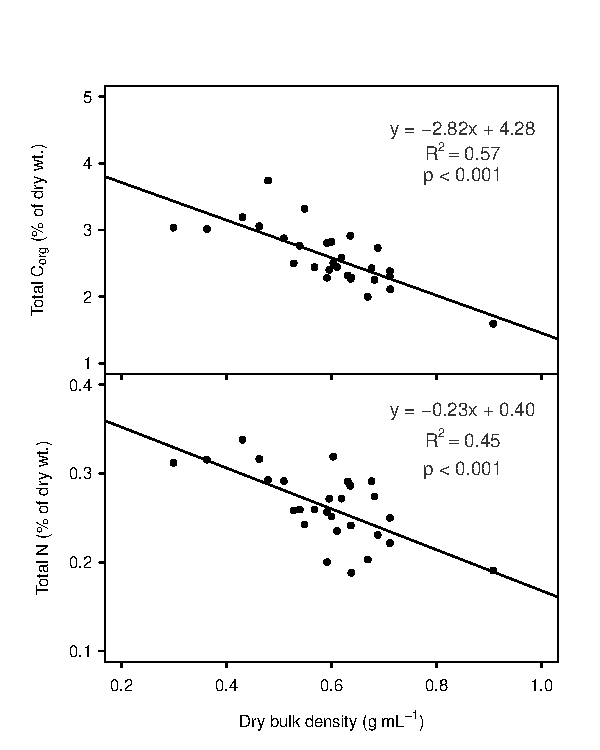
\includegraphics[width=.85\textwidth]{Figures/chapter1/fig3}
\caption[Relationships between dry bulk density and C\textsubscript{org} content (top) as well as dry bulk density and total N content (bottom) of soil samples. These models include averaged values across our five sites, two treatments and three sampled depths]{Relationships between dry bulk density and C\textsubscript{org} content (top) as well as dry bulk density and total N content (bottom) of soil samples. These models include averaged values across our five sites, two treatments and three sampled depths.}
  \label{fig:1fig3}
\end{figure}

\begin{figure}
  \centering
  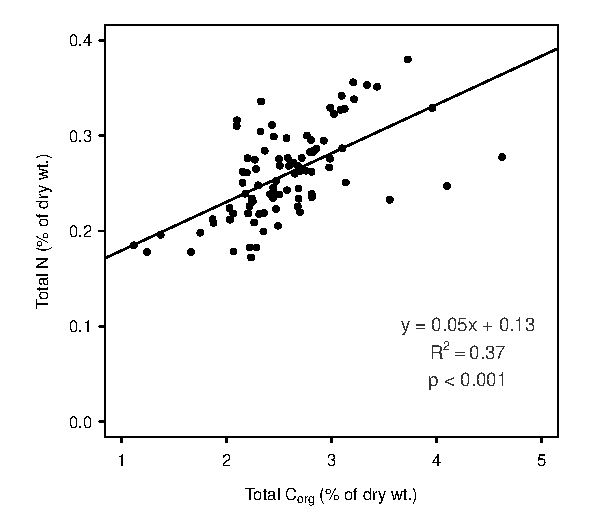
\includegraphics[width=.95\textwidth]{Figures/chapter1/fig4}
\caption[Relationship between the C\textsubscript{org} and total N content of soil samples. Values include all soil samples collected across our five sites, two treatments and three sampled depths]{Relationship between the C\textsubscript{org} and total N content of soil samples. Values include all soil samples collected across our five sites, two treatments and three sampled depths.}
  \label{fig:1fig4}
\end{figure}

\begin{figure}
  \centering
  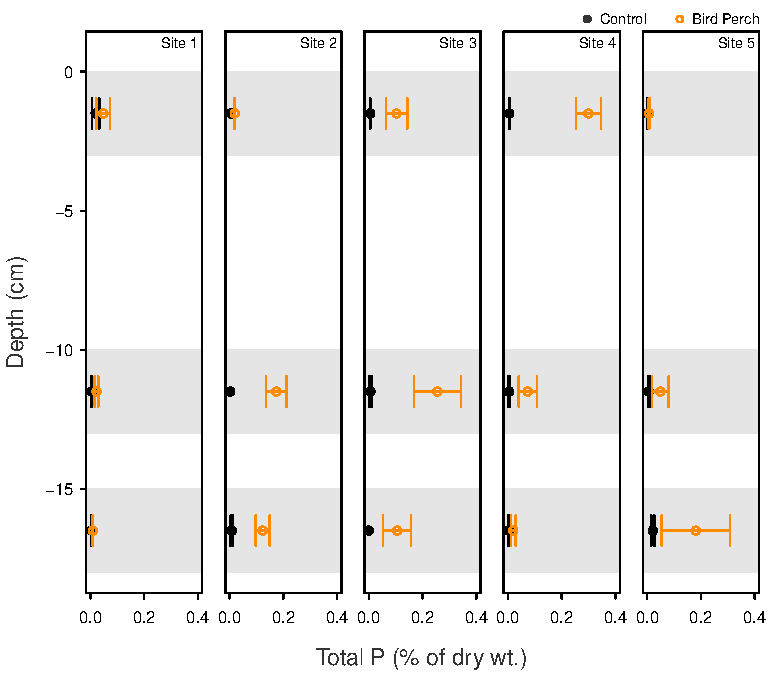
\includegraphics[width=.9\textwidth]{Figures/chapter1/fig5}
\caption[Soil phosphorus content changes with depth for bird perch treatments and controls within each experimental block. Points represent mean with horizontal error bars representing $\pm$ SE (N = 3, within-site replicates). Grey horizontal bars represent the depth range sampled and homogenized for soil analyses. The five sites (experimental blocks) are spaced 600 m apart on Cross Bank, Florida Bay]{Soil phosphorus content changes with depth for bird perch treatments and controls within each experimental block. Points represent mean with horizontal error bars representing $\pm$ SE (N = 3, within-site replicates). Grey horizontal bars represent the depth range sampled and homogenized for soil analyses. The five sites (experimental blocks) are spaced 600 m apart on Cross Bank, Florida Bay.}
  \label{fig:1fig5}
\end{figure}

\begin{figure}
  \centering
  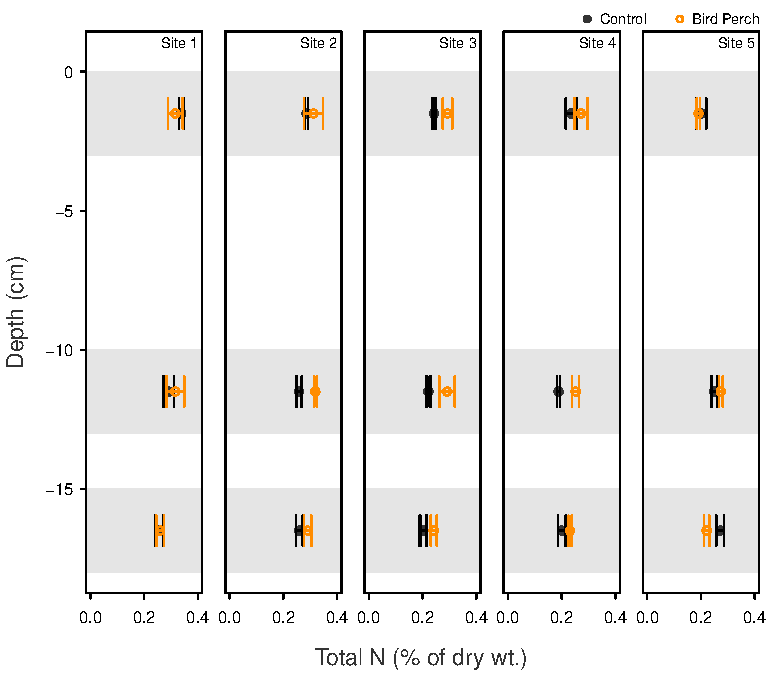
\includegraphics[width=.9\textwidth]{Figures/chapter1/fig6}
\caption[Soil nitrogen content changes with depth for bird perch treatments and controls within each experimental block. Points represent mean with horizontal error bars representing $\pm$ SE (N = 3, within-site replicates) Grey horizontal bars represent the depth range sampled and homogenized for soil analyses. The five sites (experimental blocks) are spaced 600 m apart on Cross Bank, Florida Bay]{Soil nitrogen content changes with depth for bird perch treatments and controls within each experimental block. Points represent mean with horizontal error bars representing $\pm$ SE (N = 3, within-site replicates) Grey horizontal bars represent the depth range sampled and homogenized for soil analyses. The five sites (experimental blocks) are spaced 600 m apart on Cross Bank, Florida Bay.}
  \label{fig:1fig6}
\end{figure}

\begin{figure}
  \centering
  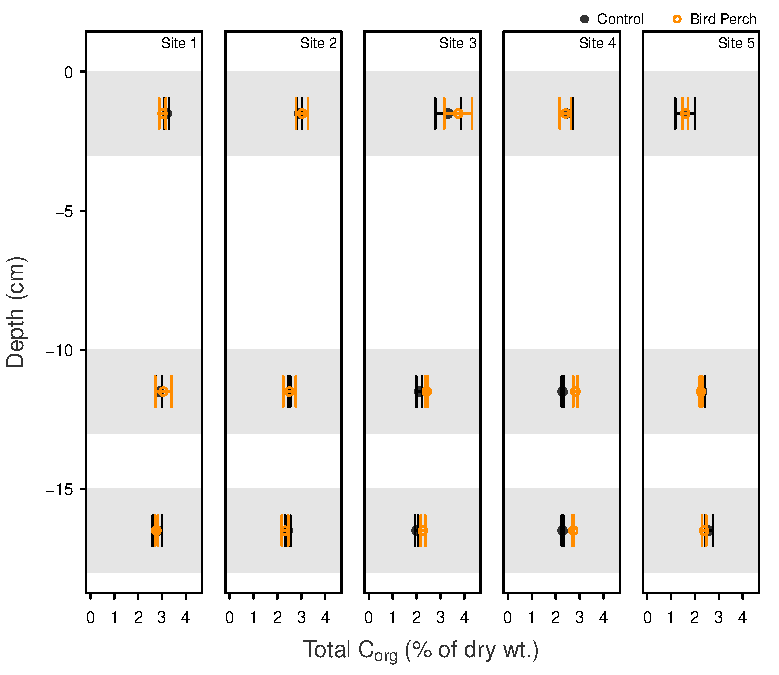
\includegraphics[width=.9\textwidth]{Figures/chapter1/fig7}
\caption[Down core profiles of soil C\textsubscript{org} content from bird perch treatments and controls within each experimental block. Points represent mean with horizontal error bars representing $\pm$ SE (N = 3, within-site replicates). Grey horizontal bars represent the depth range sampled and homogenized for soil analyses. The five sites (experimental blocks) are spaced 600 m apart on Cross Bank, Florida Bay]{Down core profiles of soil C\textsubscript{org} content from bird perch treatments and controls within each experimental block. Points represent mean with horizontal error bars representing $\pm$ SE (N = 3, within-site replicates). Grey horizontal bars represent the depth range sampled and homogenized for soil analyses. The five sites (experimental blocks) are spaced 600 m apart on Cross Bank, Florida Bay.}
  \label{fig:1fig7}
\end{figure}

\begin{figure}
  \centering
  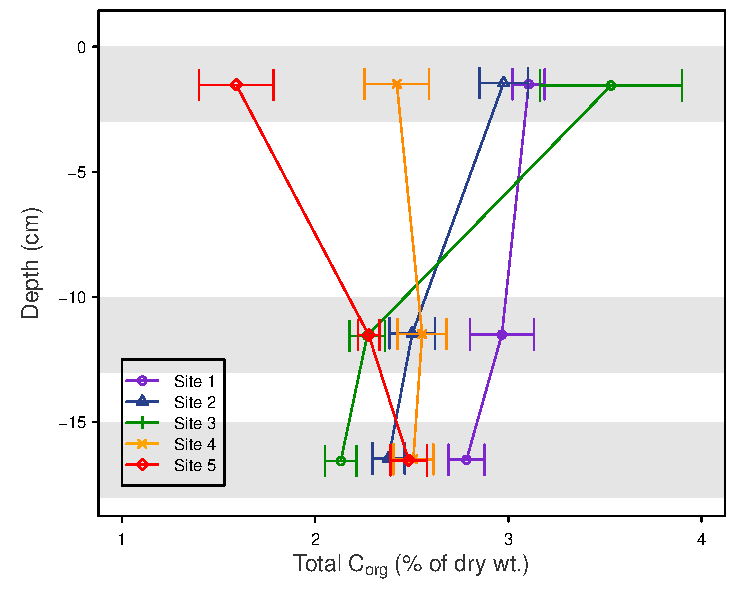
\includegraphics[width=.95\textwidth]{Figures/chapter1/fig8}
\caption[Down core profiles of soil C\textsubscript{org} content for the five sites (treated as experimental blocks), spaced 600 m apart on Cross Bank, Florida Bay. Points represent mean of samples taken from both experimental and control treatments within each site. Horizontal error bars represent $\pm$ SE (N = 6). Grey horizontal bars represent the depth range sampled and homogenized for soil analyses]{Down core profiles of soil C\textsubscript{org} content for the five sites (treated as experimental blocks), spaced 600 m apart on Cross Bank, Florida Bay. Points represent mean of samples taken from both experimental and control treatments within each site. Horizontal error bars represent $\pm$ SE (N = 6). Grey horizontal bars represent the depth range sampled and homogenized for soil analyses.}
  \label{fig:1fig8}
\end{figure}

\begin{figure}
  \centering
  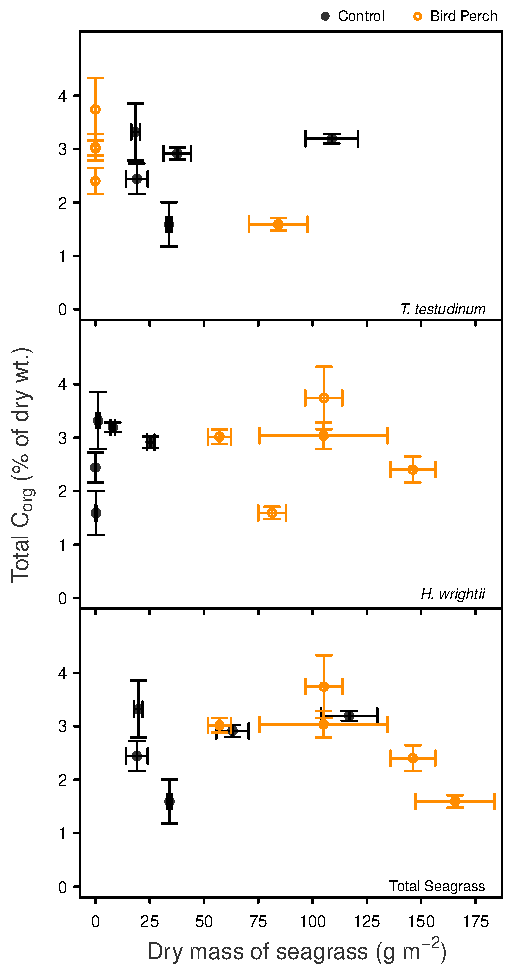
\includegraphics[width=.70\textwidth]{Figures/chapter1/fig9}
\caption[Relationship between seagrass biomass (shown as \textit{T. testudium} only, \textit{H. wrightii} only and total seagrass) and surface soil C\textsubscript{org} content across bird perch treatments and controls. Points represent mean $\pm$ SE (N = 3, within-site replicates) of above ground biomass and total C\textsubscript{org}]{Relationship between seagrass biomass (shown as \textit{T. testudium} only, \textit{H. wrightii} only and total seagrass) and surface soil C\textsubscript{org} content across bird perch treatments and controls. Points represent mean $\pm$ SE (N = 3, within-site replicates) of above ground biomass and total C\textsubscript{org}.}
  \label{fig:1fig9}
\end{figure}

\begin{figure}
  \centering
  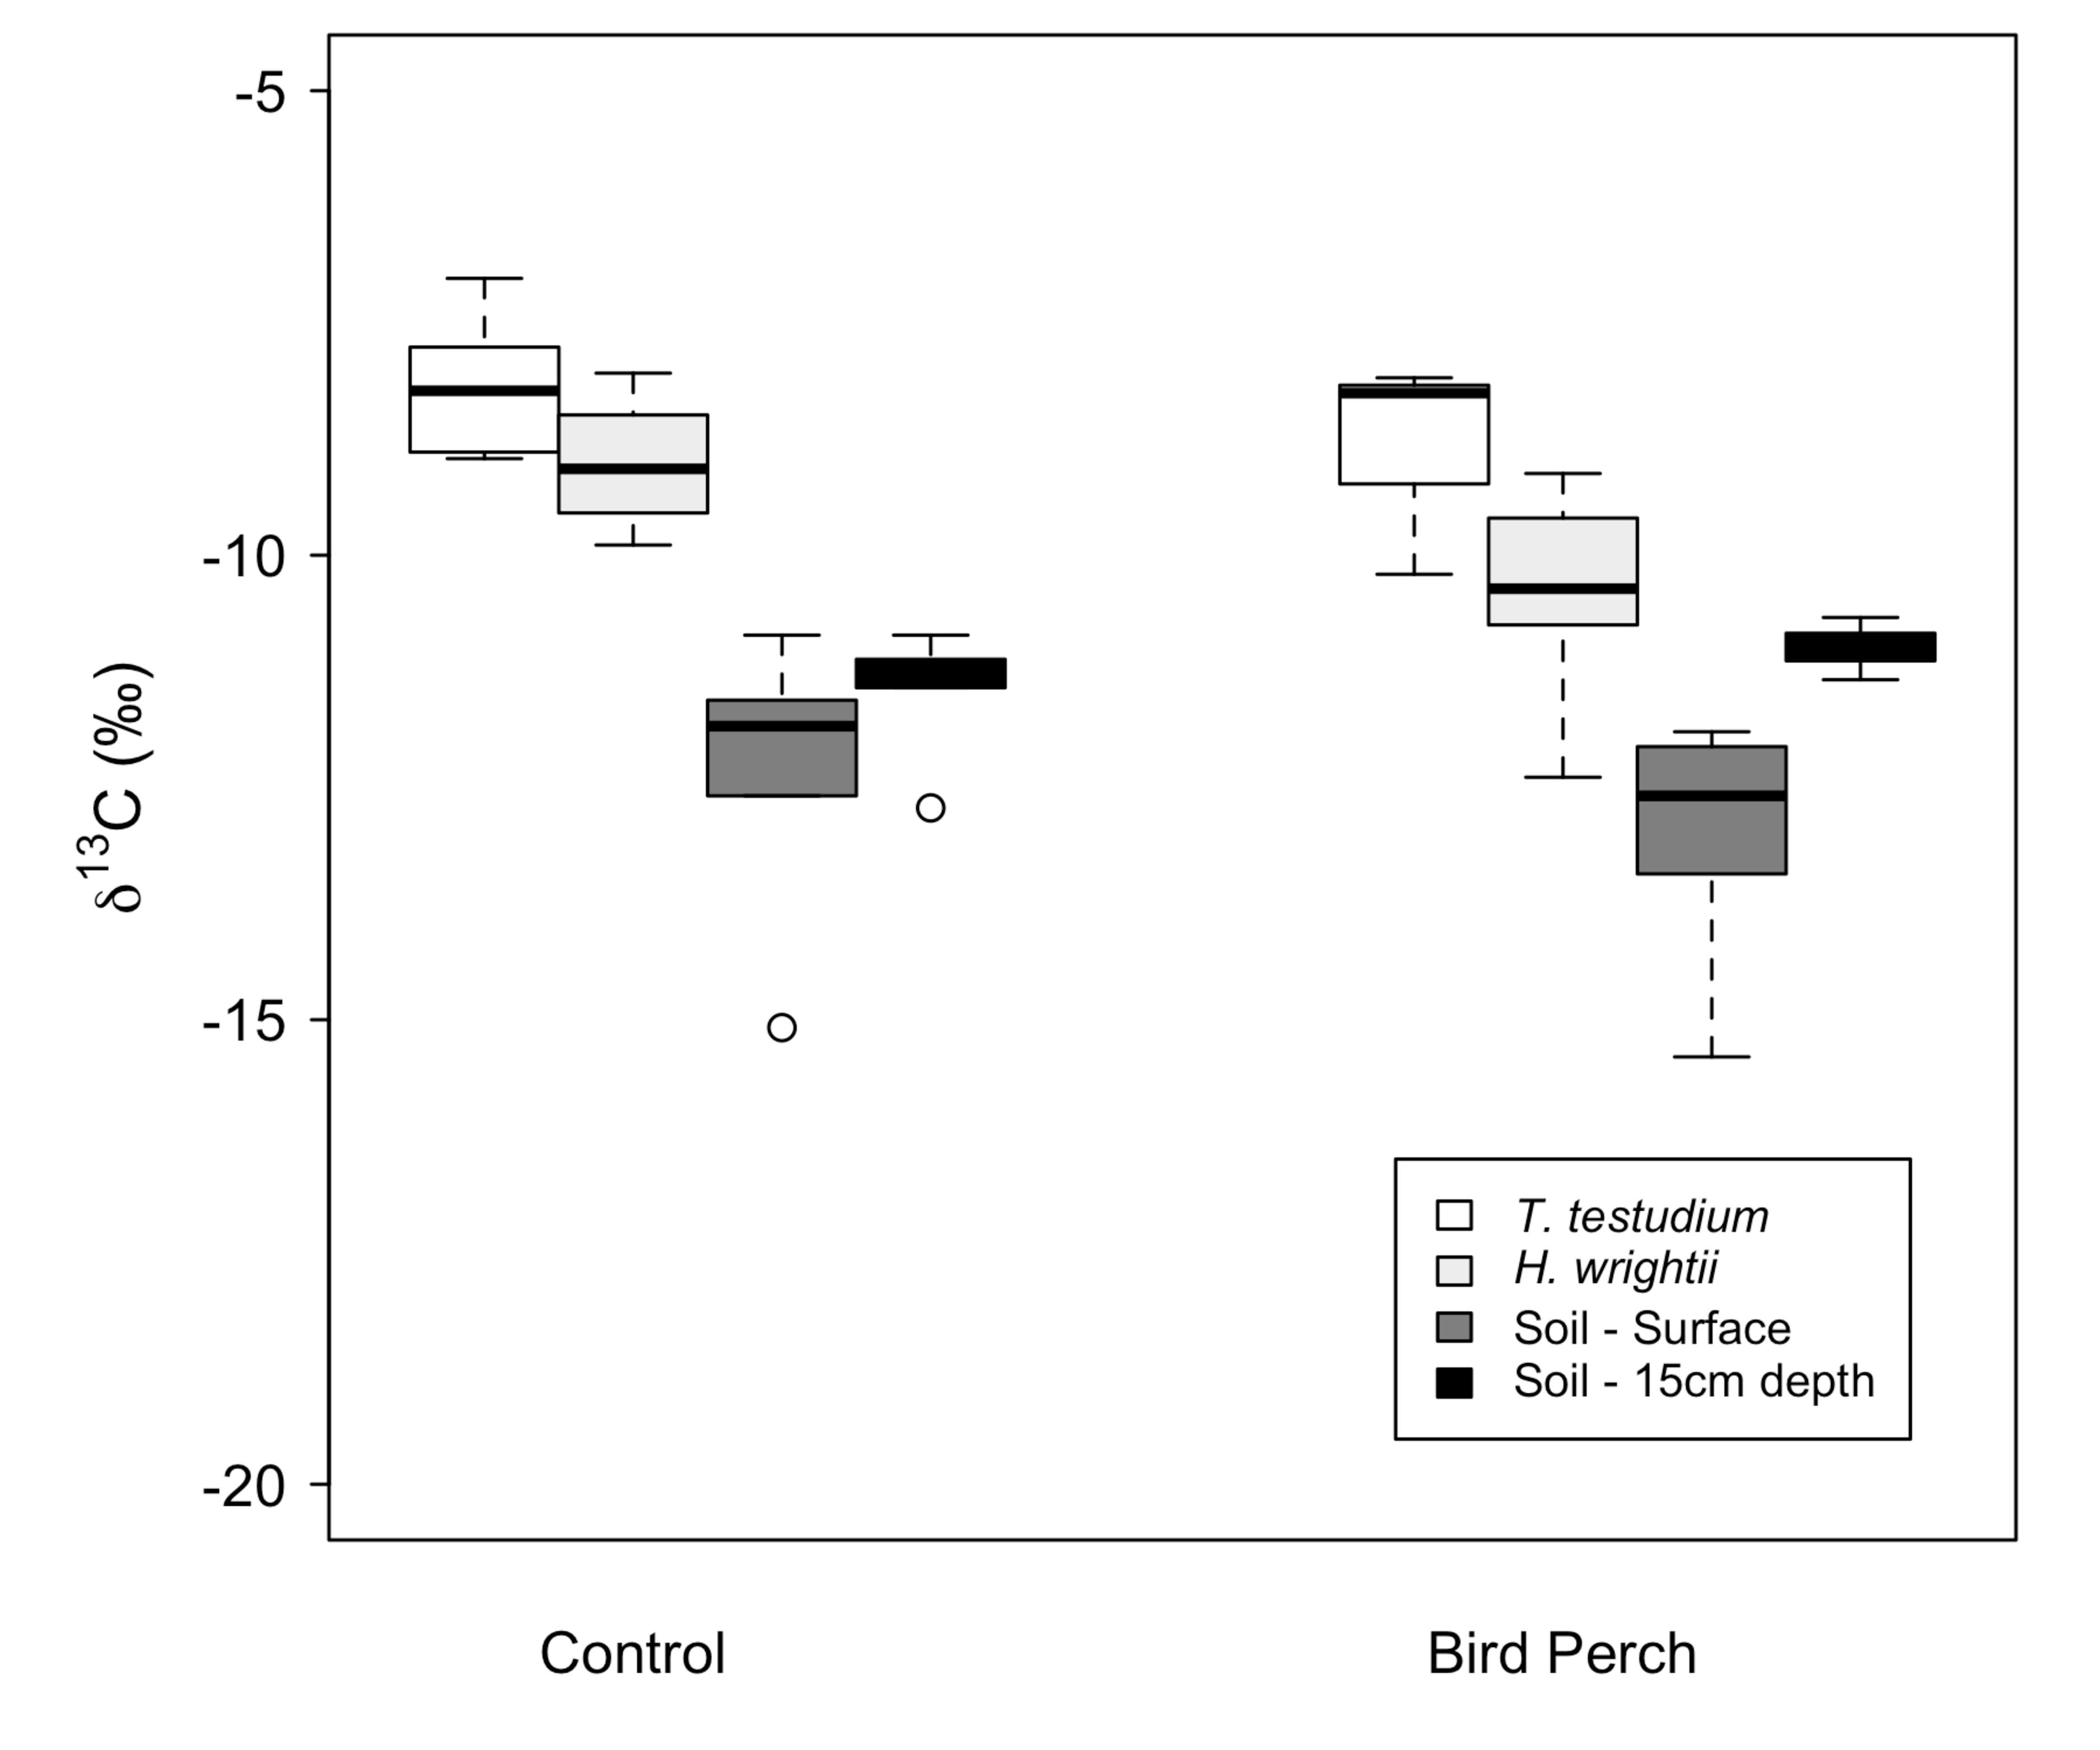
\includegraphics[width=.95\textwidth]{Figures/chapter1/fig10}
\caption[Box plots showing the distribution of the $\delta$\textsuperscript{13}C for seagrasses and underlying soils at bird perches and controls. Boxes encompass 50\% of the values, the line represents the median value, bars extend to the 95\% confidence limits, and points represent observations beyond the 95\% confidence limits (N = 5)]{Box plots showing the distribution of the $\delta$\textsuperscript{13}C for seagrasses and underlying soils at bird perches and controls. Boxes encompass 50\% of the values, the line represents the median value, bars extend to the 95\% confidence limits, and points represent observations beyond the 95\% confidence limits (N = 5). }
  \label{fig:1fig10}
\end{figure}
